\documentclass[12pt,a4paper]{article}
\usepackage[utf8]{inputenc}
\usepackage[catalan]{babel}
\usepackage{geometry}
\usepackage{graphicx}
\usepackage{float}
\usepackage{array}
\usepackage{booktabs}
\usepackage{longtable}

\geometry{margin=2.5cm}

\title{Informe de Resultats Acadèmics\\
\small Grau en Matemàtiques\\
\small Doble Grau en Matemàtiques i en Enginyeria Telemàtica\\
\small Doble Grau en Matemàtiques i en Enginyeria Informàtica\\
\small Doble Grau en Física i Matemàtiques}
\author{Sergio López Ureña - Coordinació 2o curs}
\date{\today}

\begin{document}

\maketitle
\tableofcontents
\newpage


\section{Primer Quadrimestre - Primera Convocatòria}


\subsection{34154 - Programació matemàtica - Grup A}


\begin{table}[H]
\centering
\caption{34154 - Programació matemàtica - Grup A - Convocatòria 1}
\begin{tabular}{|l|c|c|}
\hline
\textbf{Resultat} & \textbf{Estudiants} & \textbf{Percentatge} \\
\hline
No presentat & 15 & 23.8\% \\
Suspès & 10 & 15.9\% \\
Aprovat & 9 & 14.3\% \\
Notable & 7 & 11.1\% \\
Excel·lent & 11 & 17.5\% \\
Matrícula d'Honor & 11 & 17.5\% \\
\hline
\textbf{Total} & \textbf{63} & \textbf{100.0\%} \\
\hline
\end{tabular}
\end{table}

\begin{figure}[H]
\centering
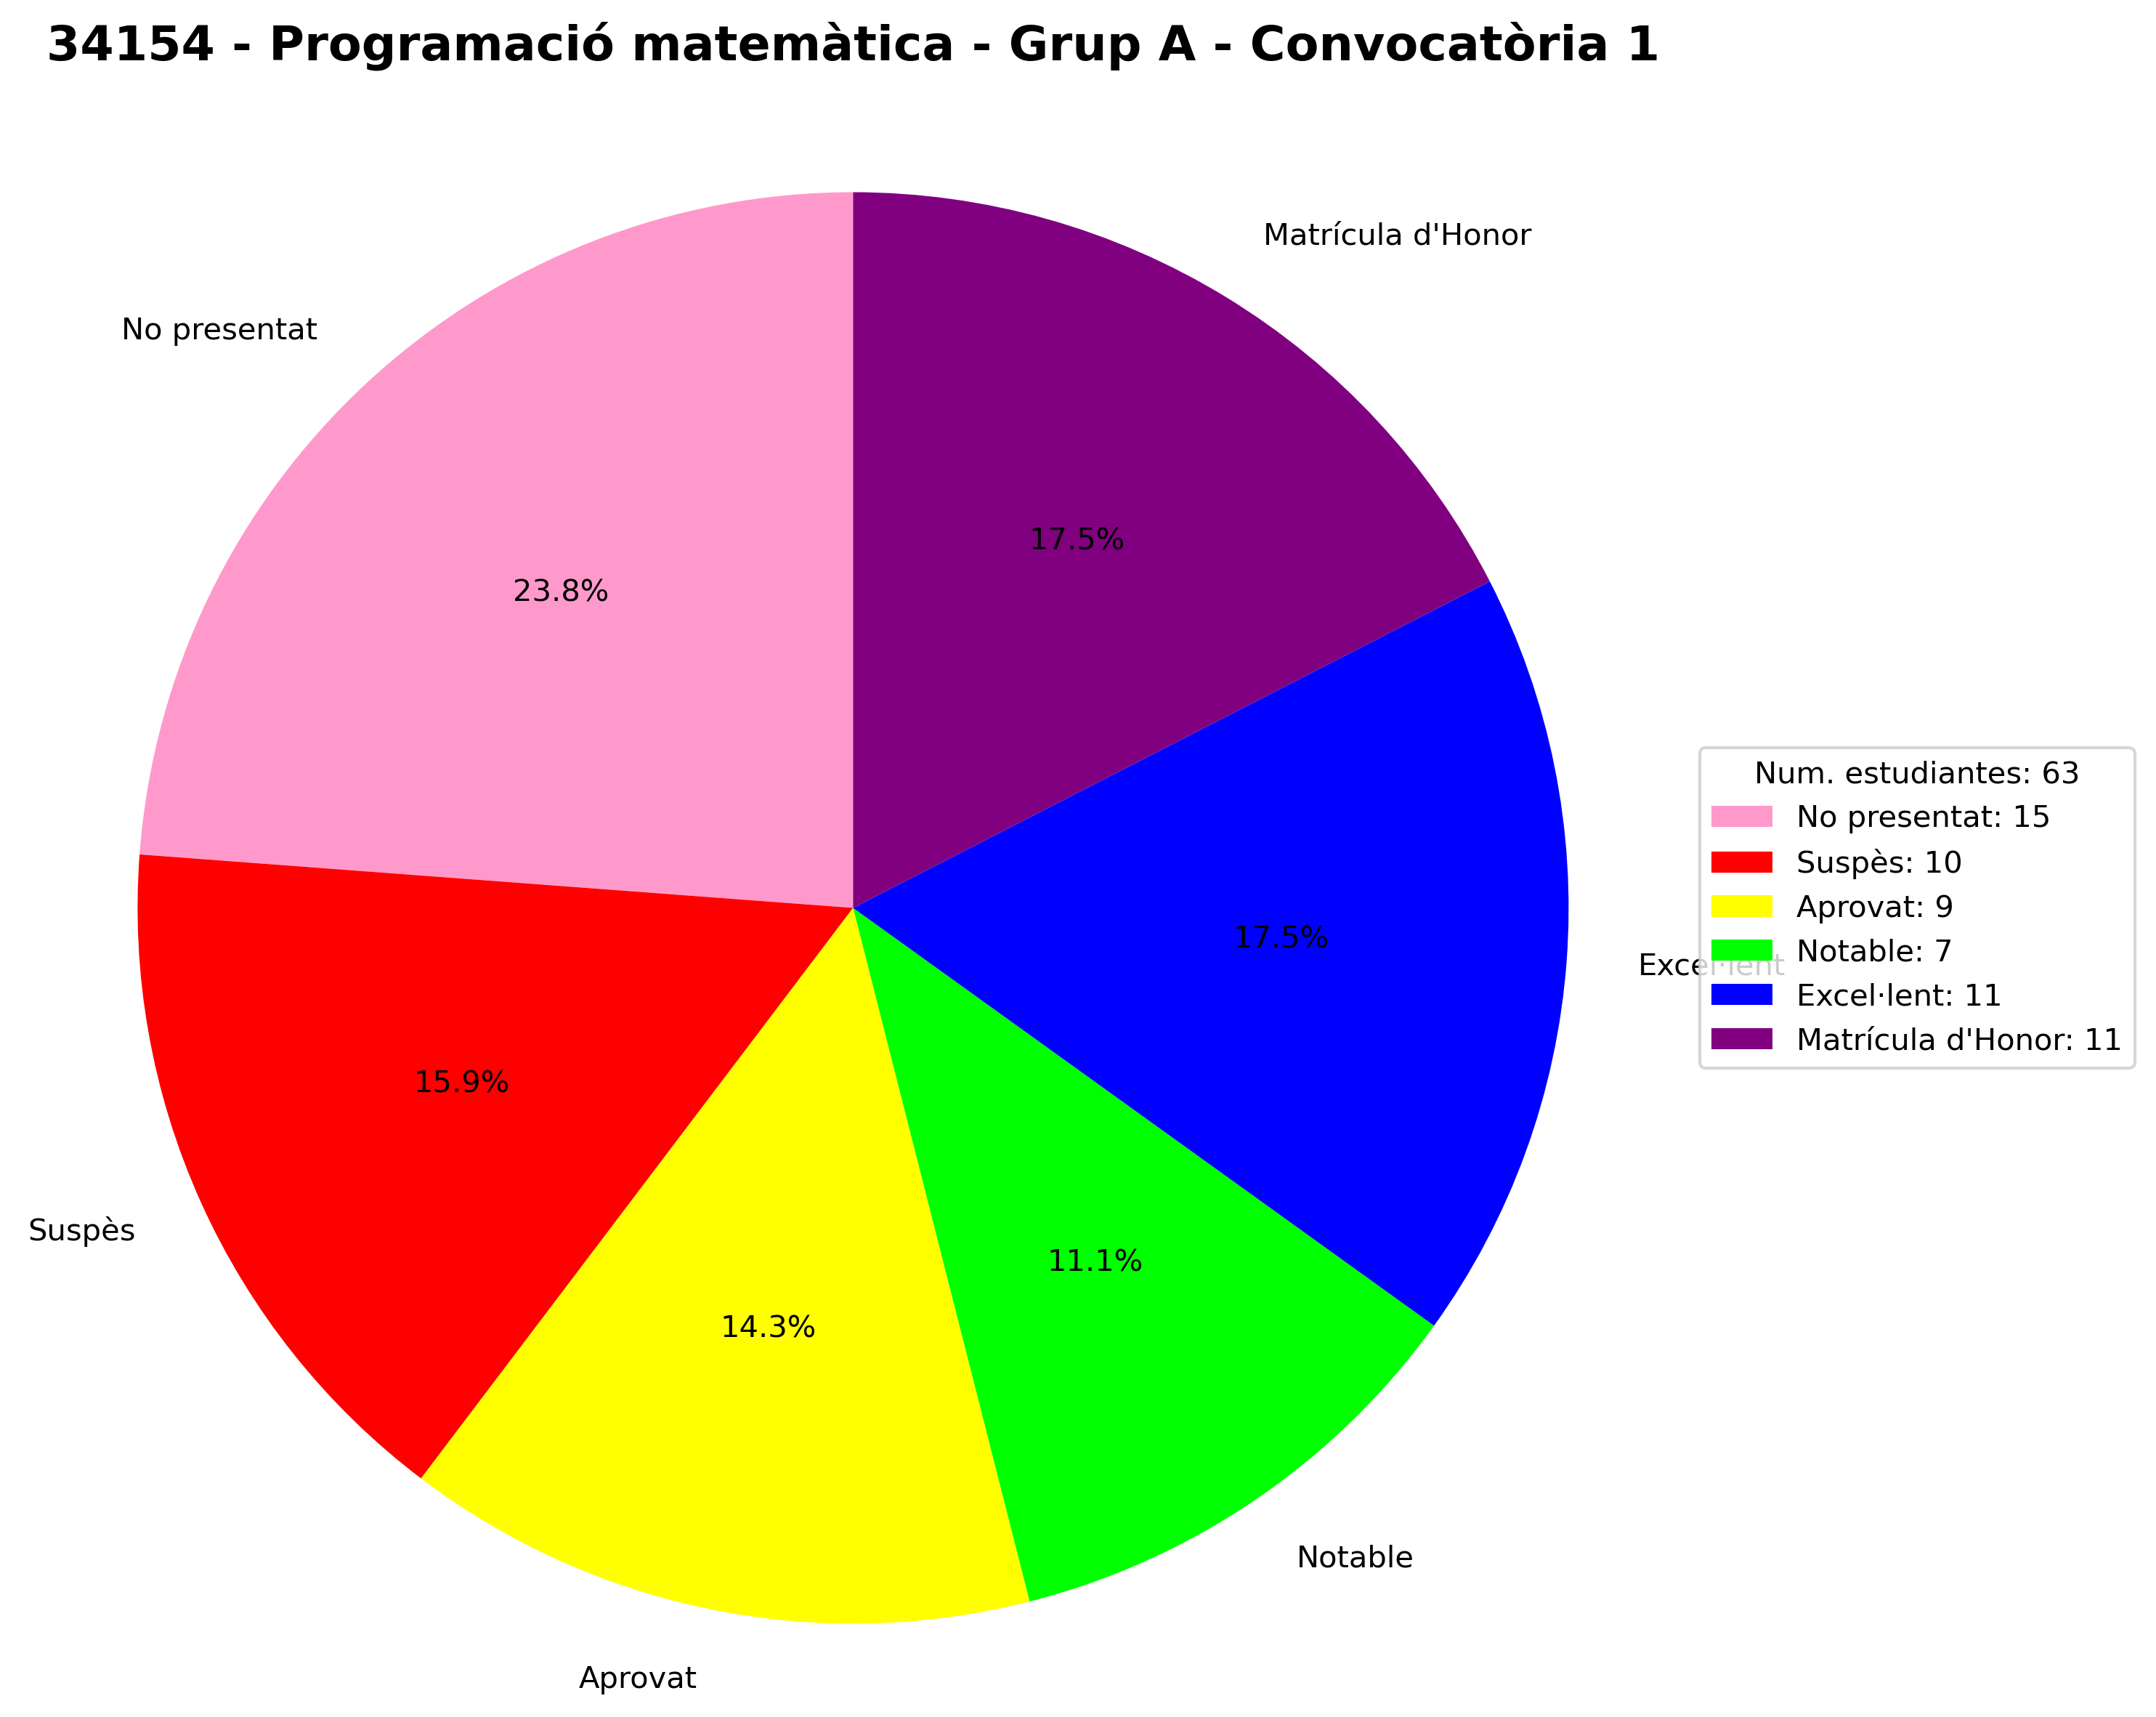
\includegraphics[width=0.8\textwidth]{graficos/34154_A_1Q1_0.png}
\caption{34154 - Programació matemàtica - Grup A - Convocatòria 1}
\end{figure}

\newpage


\section{Primer Quadrimestre - Segona Convocatòria}


\subsection{34154 - Programació matemàtica - Grup A}


\begin{table}[H]
\centering
\caption{34154 - Programació matemàtica - Grup A - Convocatòria 2}
\begin{tabular}{|l|c|c|}
\hline
\textbf{Resultat} & \textbf{Estudiants} & \textbf{Percentatge} \\
\hline
No presentat & 9 & 18.8\% \\
Suspès & 11 & 22.9\% \\
Aprovat & 5 & 10.4\% \\
Notable & 6 & 12.5\% \\
Excel·lent & 10 & 20.8\% \\
Matrícula d'Honor & 7 & 14.6\% \\
\hline
\textbf{Total} & \textbf{48} & \textbf{100.0\%} \\
\hline
\end{tabular}
\end{table}

\begin{figure}[H]
\centering
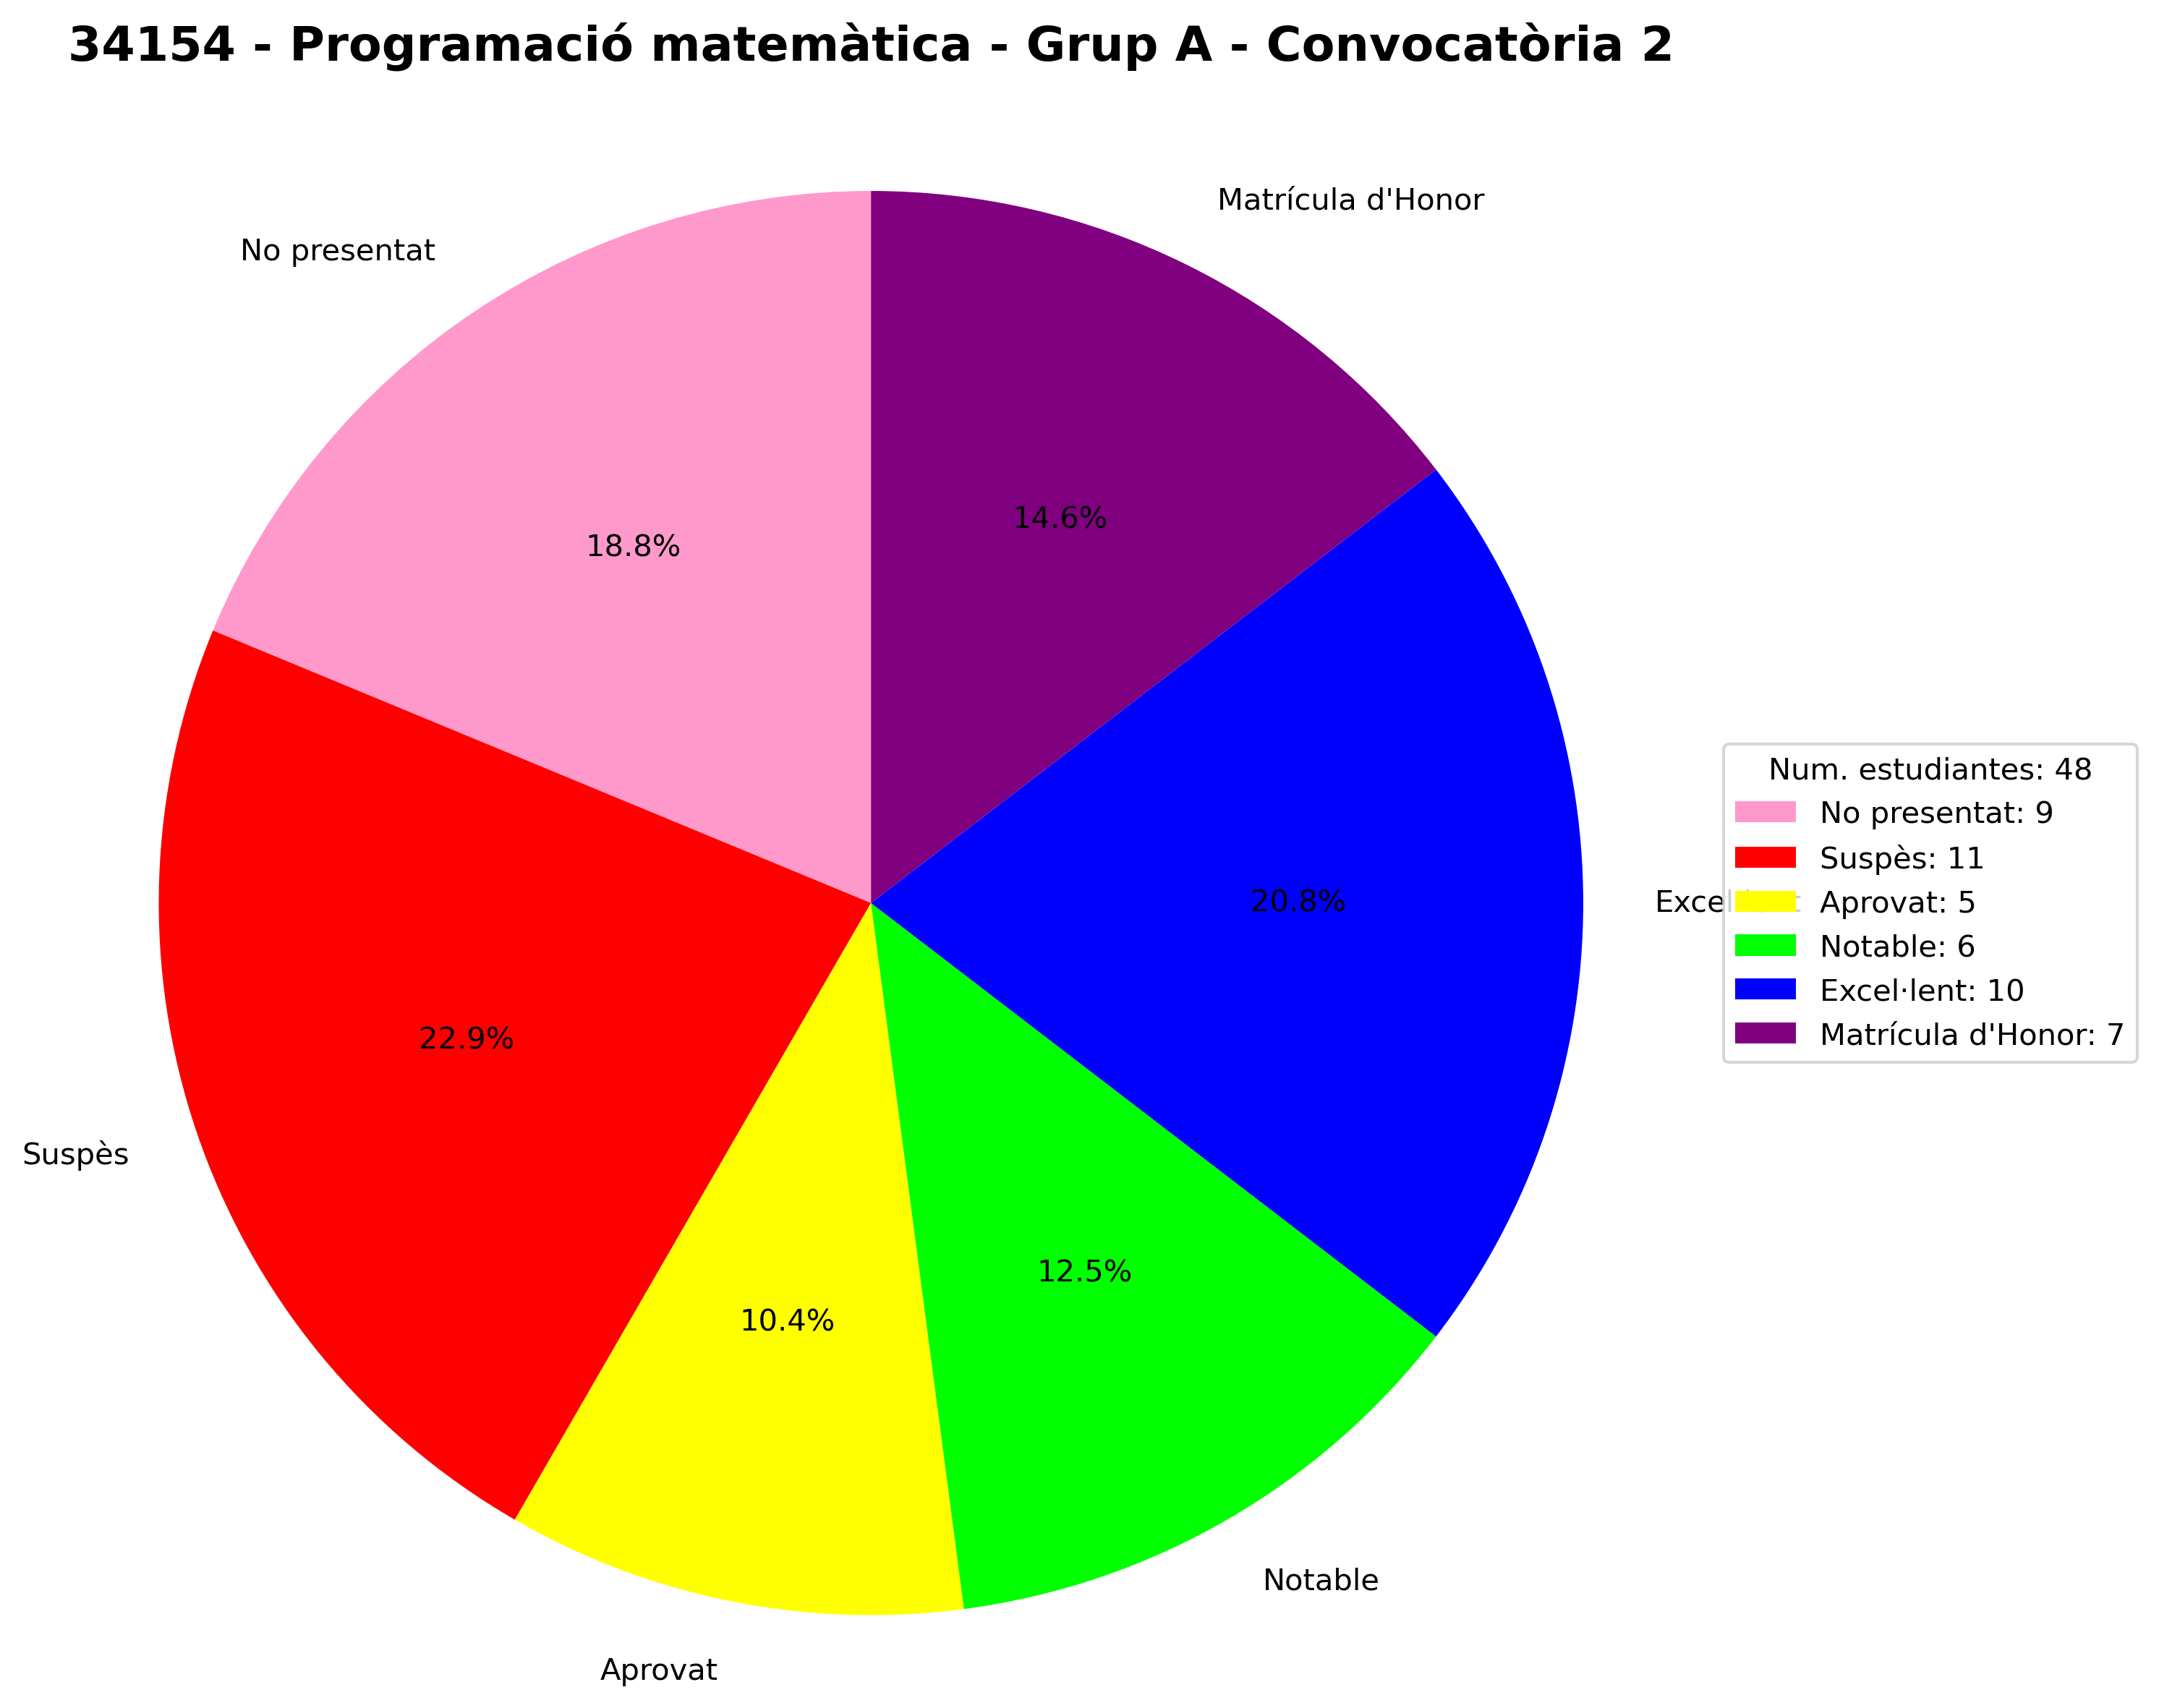
\includegraphics[width=0.8\textwidth]{graficos/34154_A_1Q2.png}
\caption{34154 - Programació matemàtica - Grup A - Convocatòria 2}
\end{figure}

\newpage


\section{Segon Quadrimestre - Primera Convocatòria}


\subsection{34155 - Àlgebra lineal i geometria II - Grup A}


\begin{table}[H]
\centering
\caption{34155 - Àlgebra lineal i geometria II - Grup A - Convocatòria 1}
\begin{tabular}{|l|c|c|}
\hline
\textbf{Resultat} & \textbf{Estudiants} & \textbf{Percentatge} \\
\hline
No presentat & 8 & 13.3\% \\
Suspès & 12 & 20.0\% \\
Aprovat & 12 & 20.0\% \\
Notable & 8 & 13.3\% \\
Excel·lent & 5 & 8.3\% \\
Matrícula d'Honor & 15 & 25.0\% \\
\hline
\textbf{Total} & \textbf{60} & \textbf{100.0\%} \\
\hline
\end{tabular}
\end{table}

\begin{figure}[H]
\centering
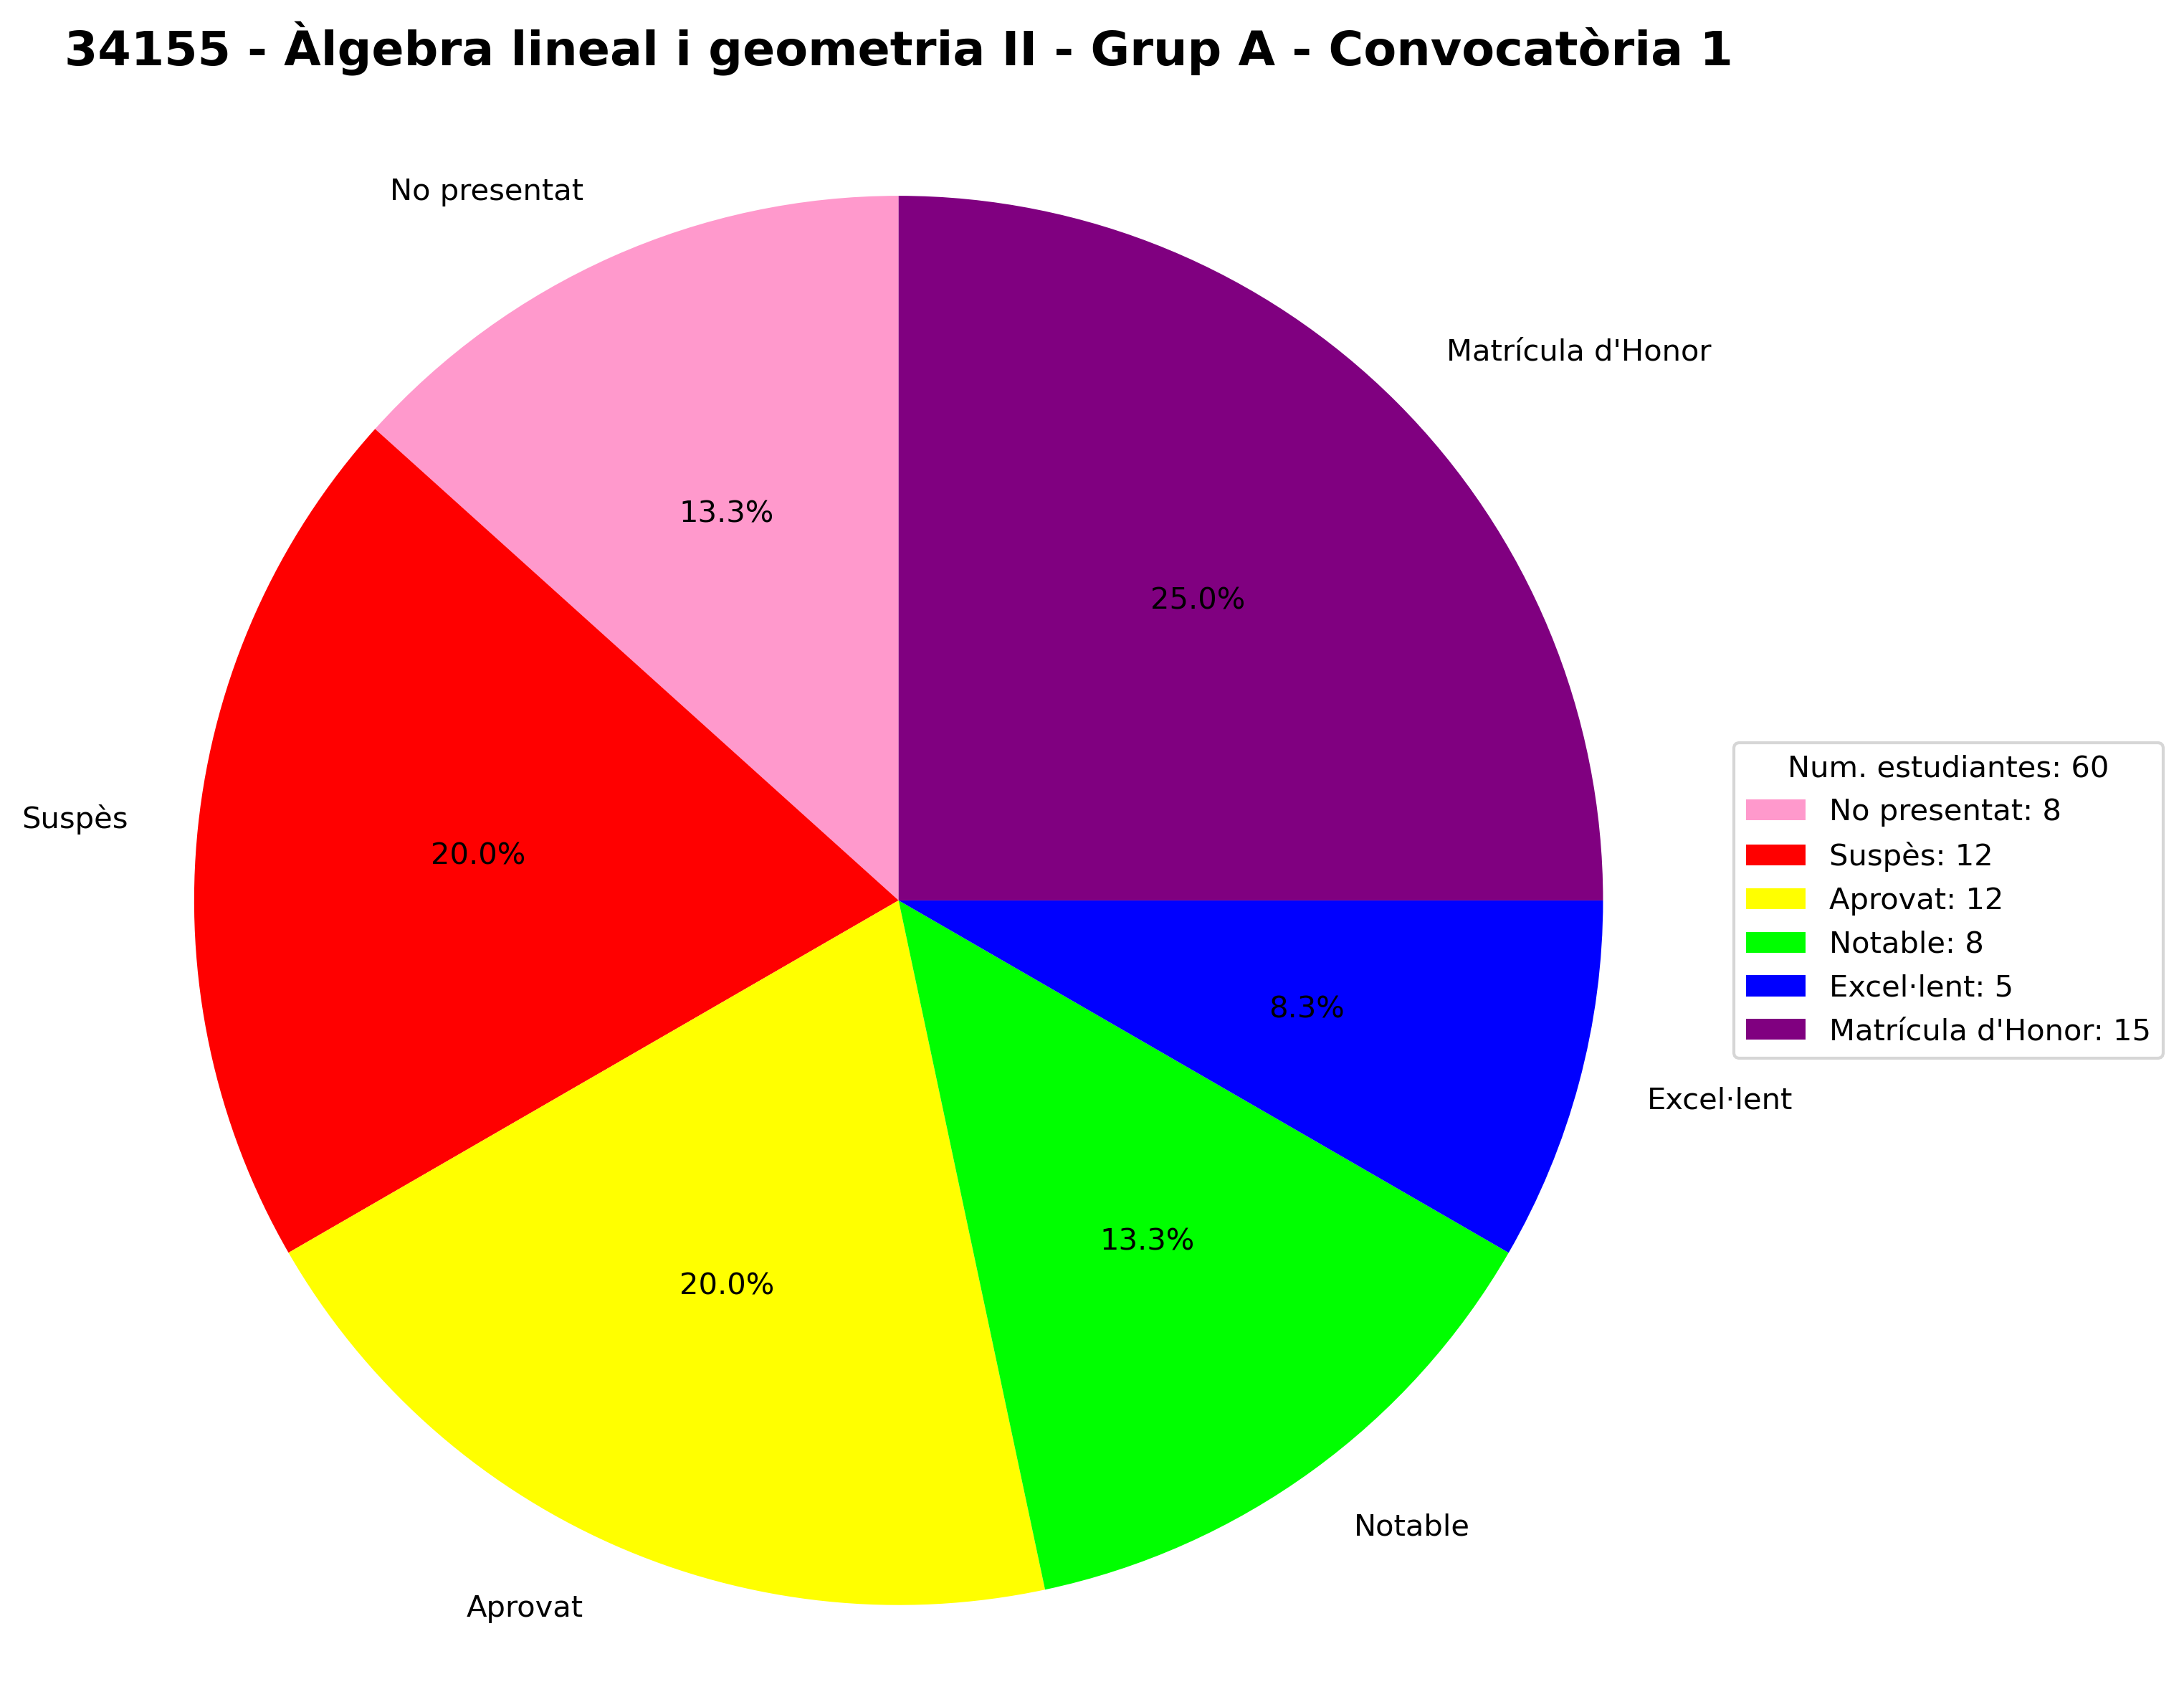
\includegraphics[width=0.8\textwidth]{graficos/34155_A_2Q1.png}
\caption{34155 - Àlgebra lineal i geometria II - Grup A - Convocatòria 1}
\end{figure}

\newpage


\section{Segon Quadrimestre - Segona Convocatòria}


\subsection{34155 - Àlgebra lineal i geometria II - Grup A}


\begin{table}[H]
\centering
\caption{34155 - Àlgebra lineal i geometria II - Grup A - Convocatòria 2}
\begin{tabular}{|l|c|c|}
\hline
\textbf{Resultat} & \textbf{Estudiants} & \textbf{Percentatge} \\
\hline
No presentat & 3 & 42.9\% \\
Aprovat & 2 & 28.6\% \\
Notable & 1 & 14.3\% \\
Excel·lent & 1 & 14.3\% \\
\hline
\textbf{Total} & \textbf{7} & \textbf{100.0\%} \\
\hline
\end{tabular}
\end{table}

\begin{figure}[H]
\centering
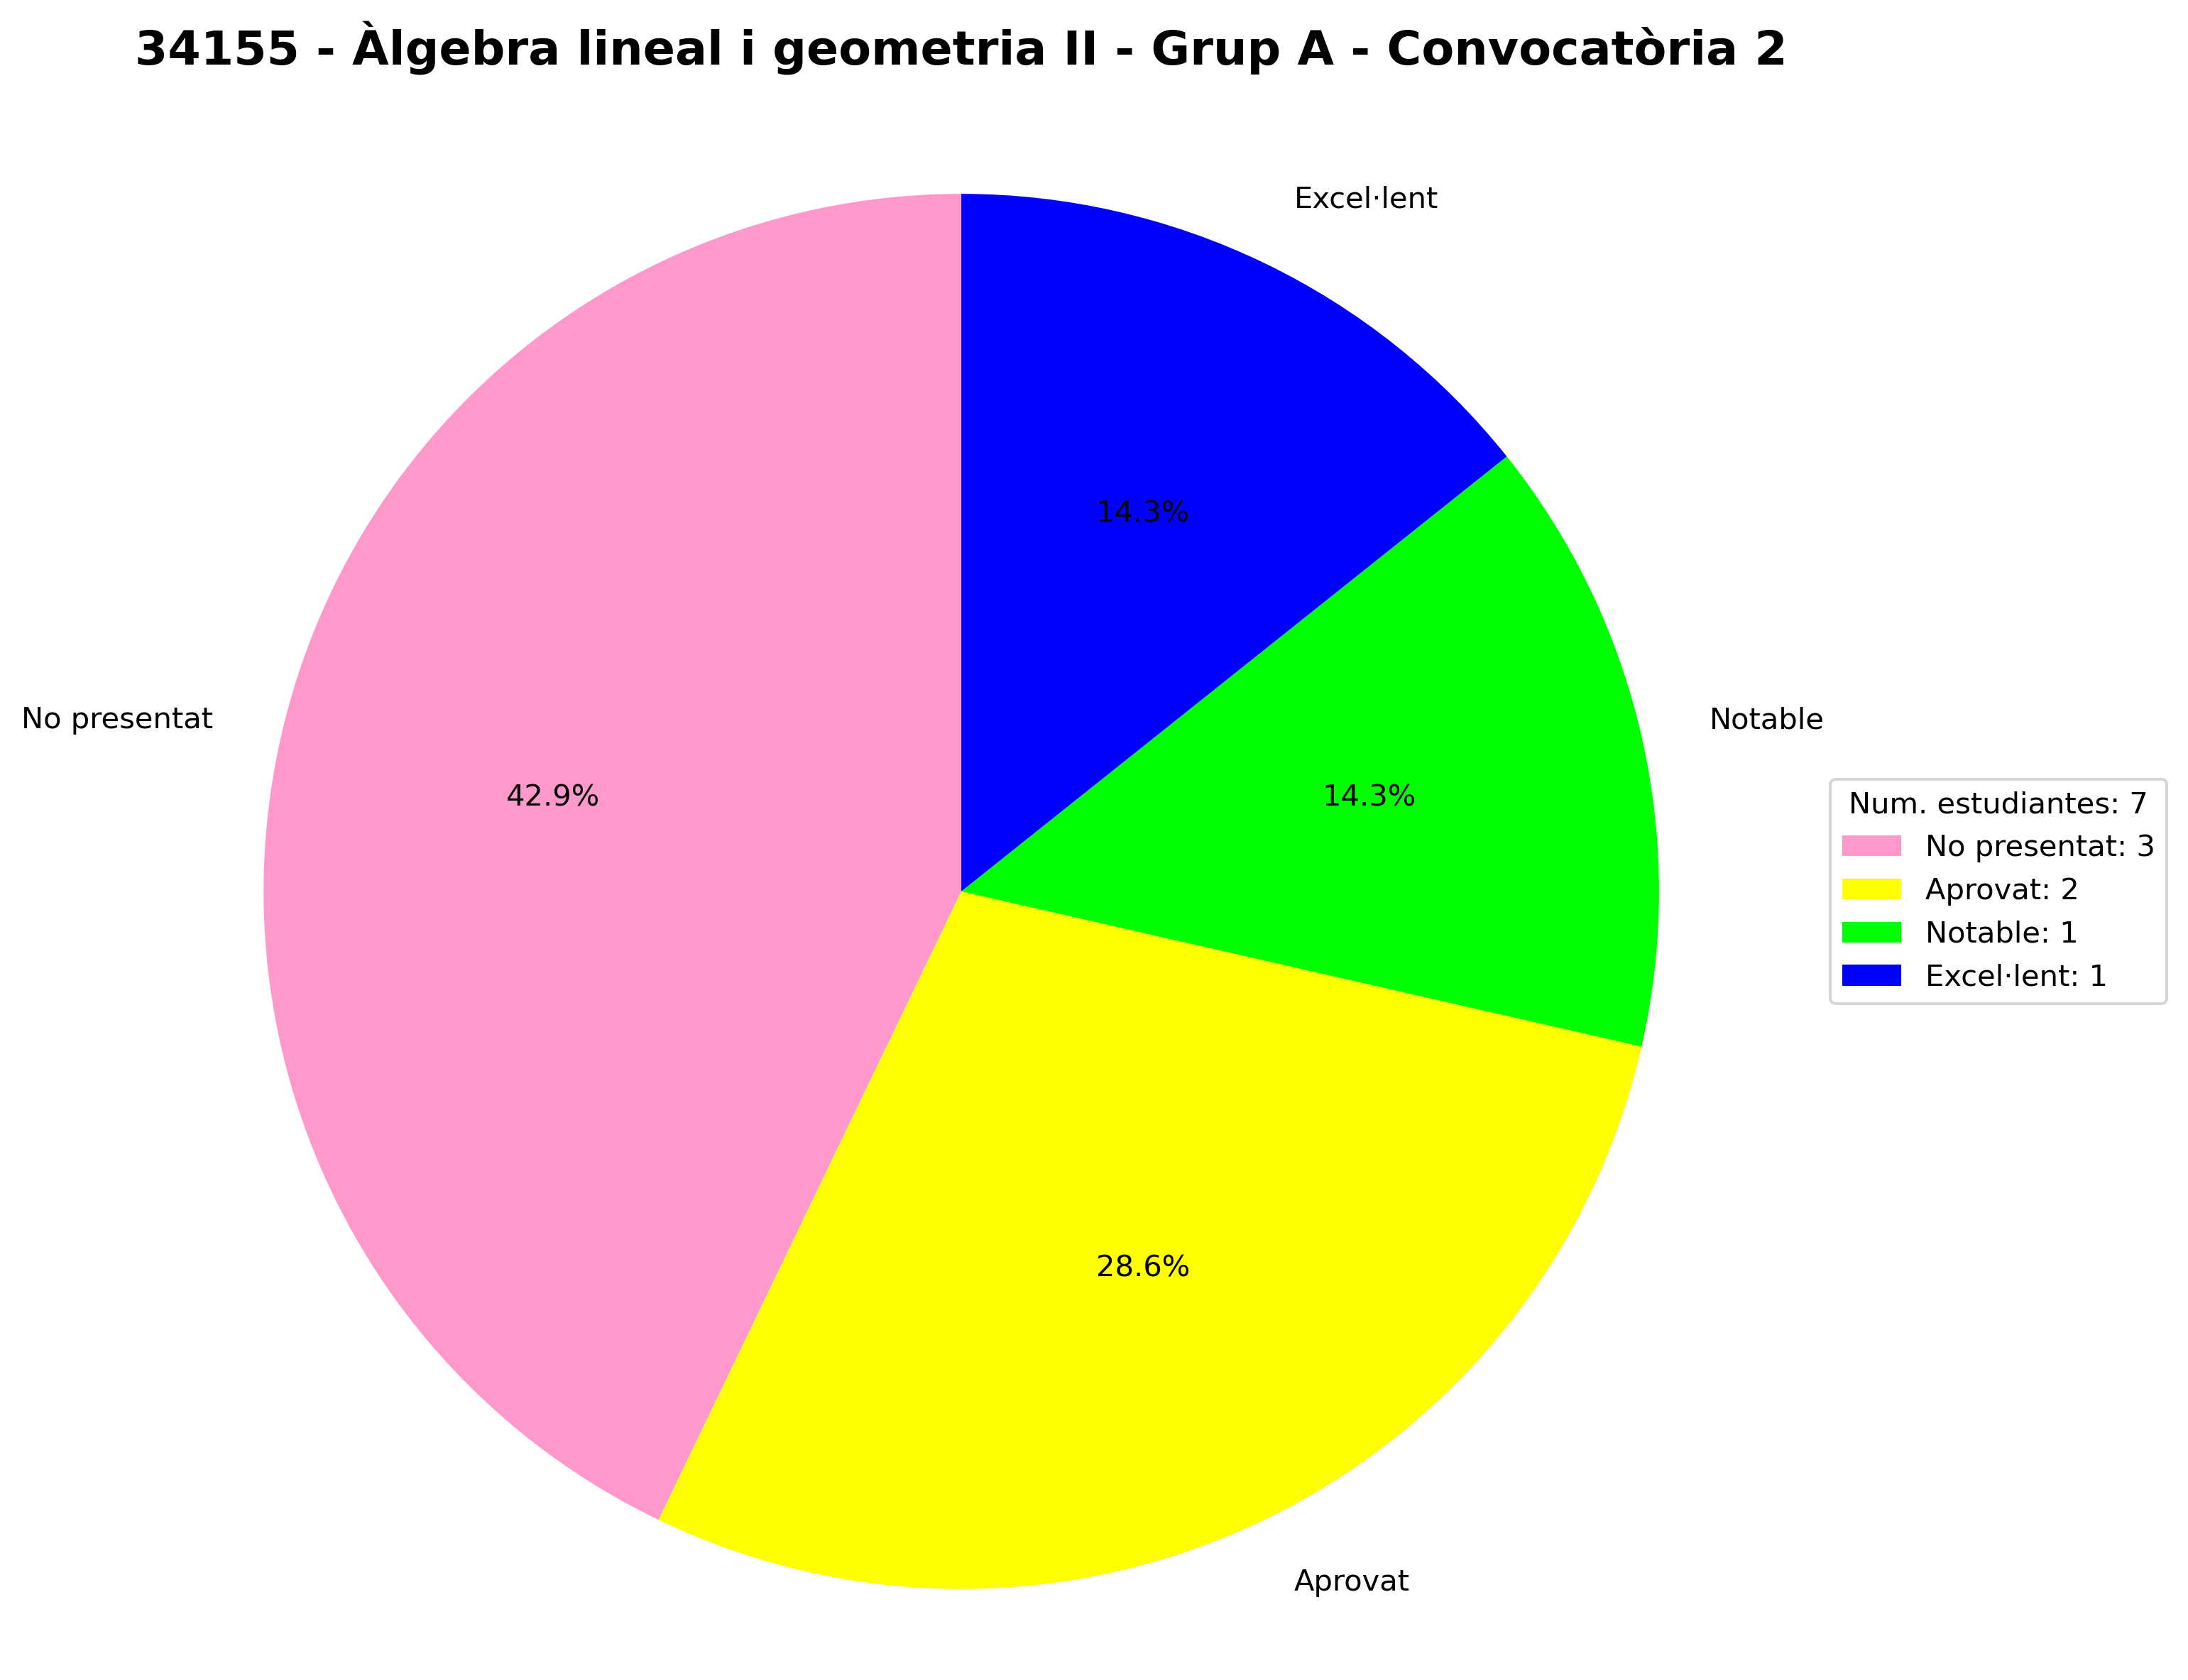
\includegraphics[width=0.8\textwidth]{graficos/34155_A_2Q2.png}
\caption{34155 - Àlgebra lineal i geometria II - Grup A - Convocatòria 2}
\end{figure}

\newpage


\section{Assignatures Anuals - Primera Convocatòria}


\subsection{34156 - Anàlisi matemàtica II - Grup A}


\begin{table}[H]
\centering
\caption{34156 - Anàlisi matemàtica II - Grup A - Convocatòria 1}
\begin{tabular}{|l|c|c|}
\hline
\textbf{Resultat} & \textbf{Estudiants} & \textbf{Percentatge} \\
\hline
No presentat & 9 & 13.2\% \\
Suspès & 12 & 17.6\% \\
Aprovat & 10 & 14.7\% \\
Notable & 9 & 13.2\% \\
Excel·lent & 16 & 23.5\% \\
Matrícula d'Honor & 12 & 17.6\% \\
\hline
\textbf{Total} & \textbf{68} & \textbf{100.0\%} \\
\hline
\end{tabular}
\end{table}

\begin{figure}[H]
\centering
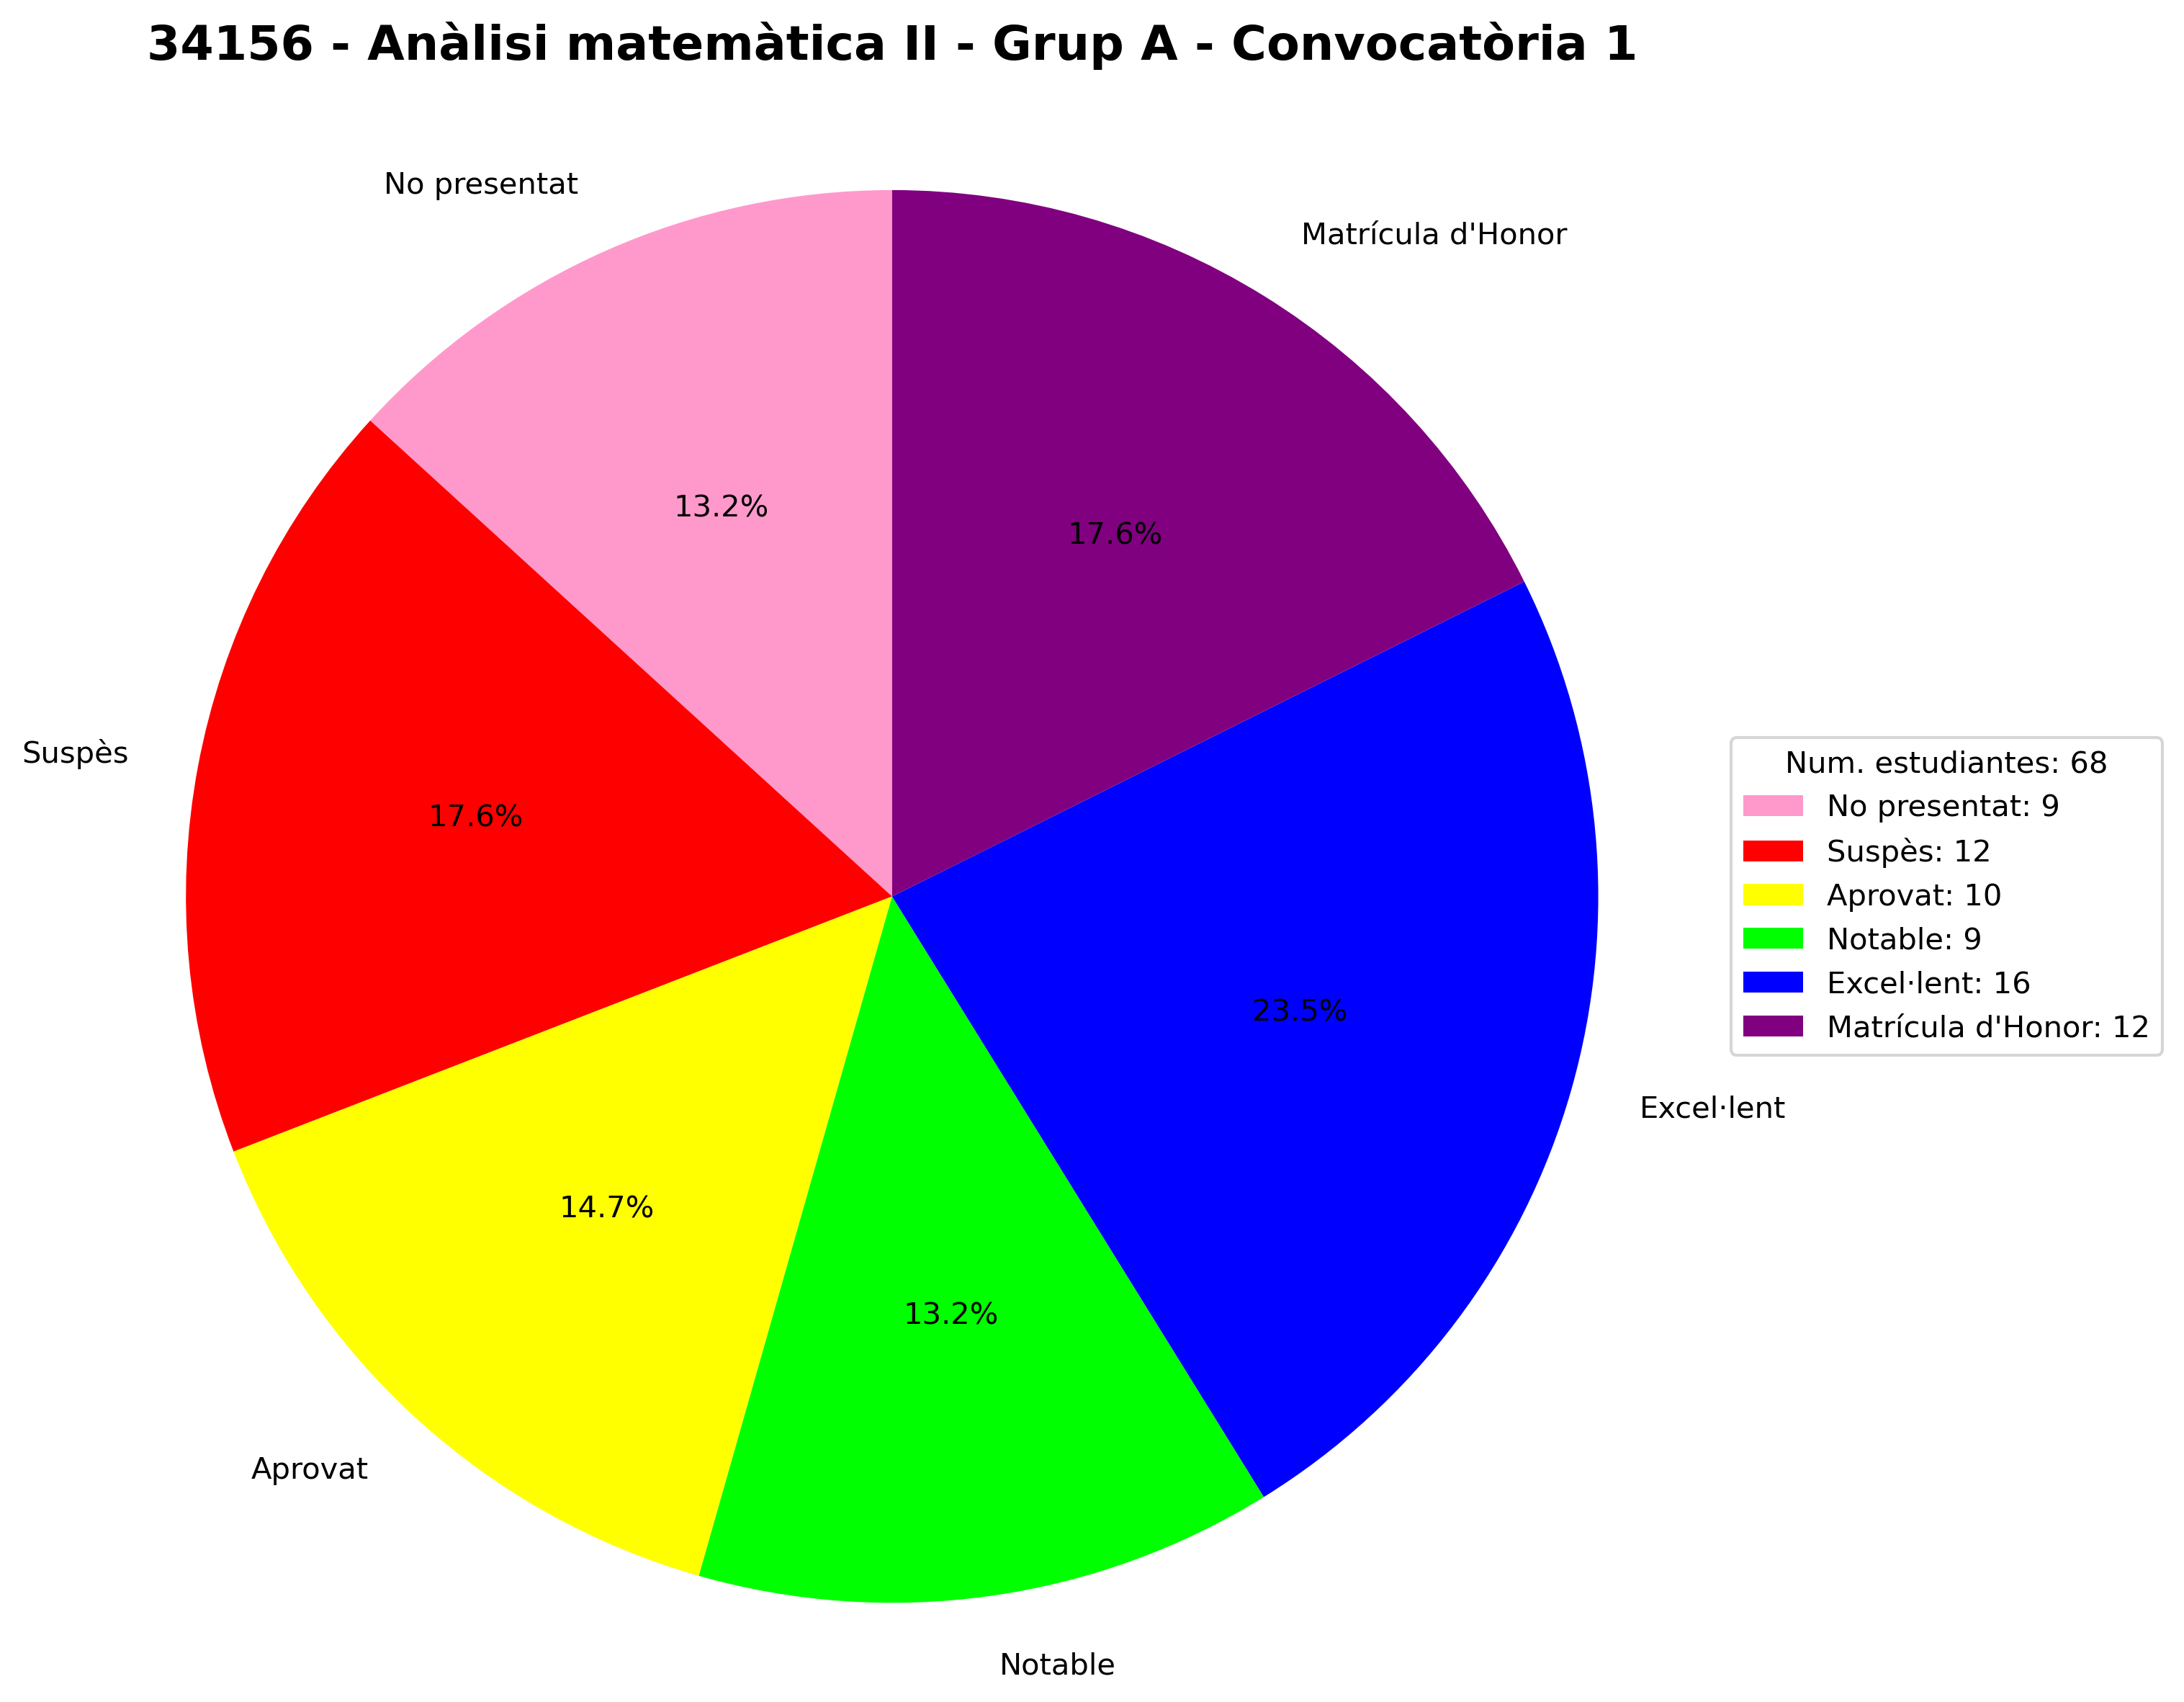
\includegraphics[width=0.8\textwidth]{graficos/34156_A_A1.png}
\caption{34156 - Anàlisi matemàtica II - Grup A - Convocatòria 1}
\end{figure}

\newpage


\section{Assignatures Anuals - Segona Convocatòria}


\subsection{34156 - Anàlisi matemàtica II - Grup A}


\begin{table}[H]
\centering
\caption{34156 - Anàlisi matemàtica II - Grup A - Convocatòria 2}
\begin{tabular}{|l|c|c|}
\hline
\textbf{Resultat} & \textbf{Estudiants} & \textbf{Percentatge} \\
\hline
No presentat & 10 & 23.3\% \\
Suspès & 6 & 14.0\% \\
Aprovat & 4 & 9.3\% \\
Notable & 9 & 20.9\% \\
Excel·lent & 4 & 9.3\% \\
Matrícula d'Honor & 10 & 23.3\% \\
\hline
\textbf{Total} & \textbf{43} & \textbf{100.0\%} \\
\hline
\end{tabular}
\end{table}

\begin{figure}[H]
\centering
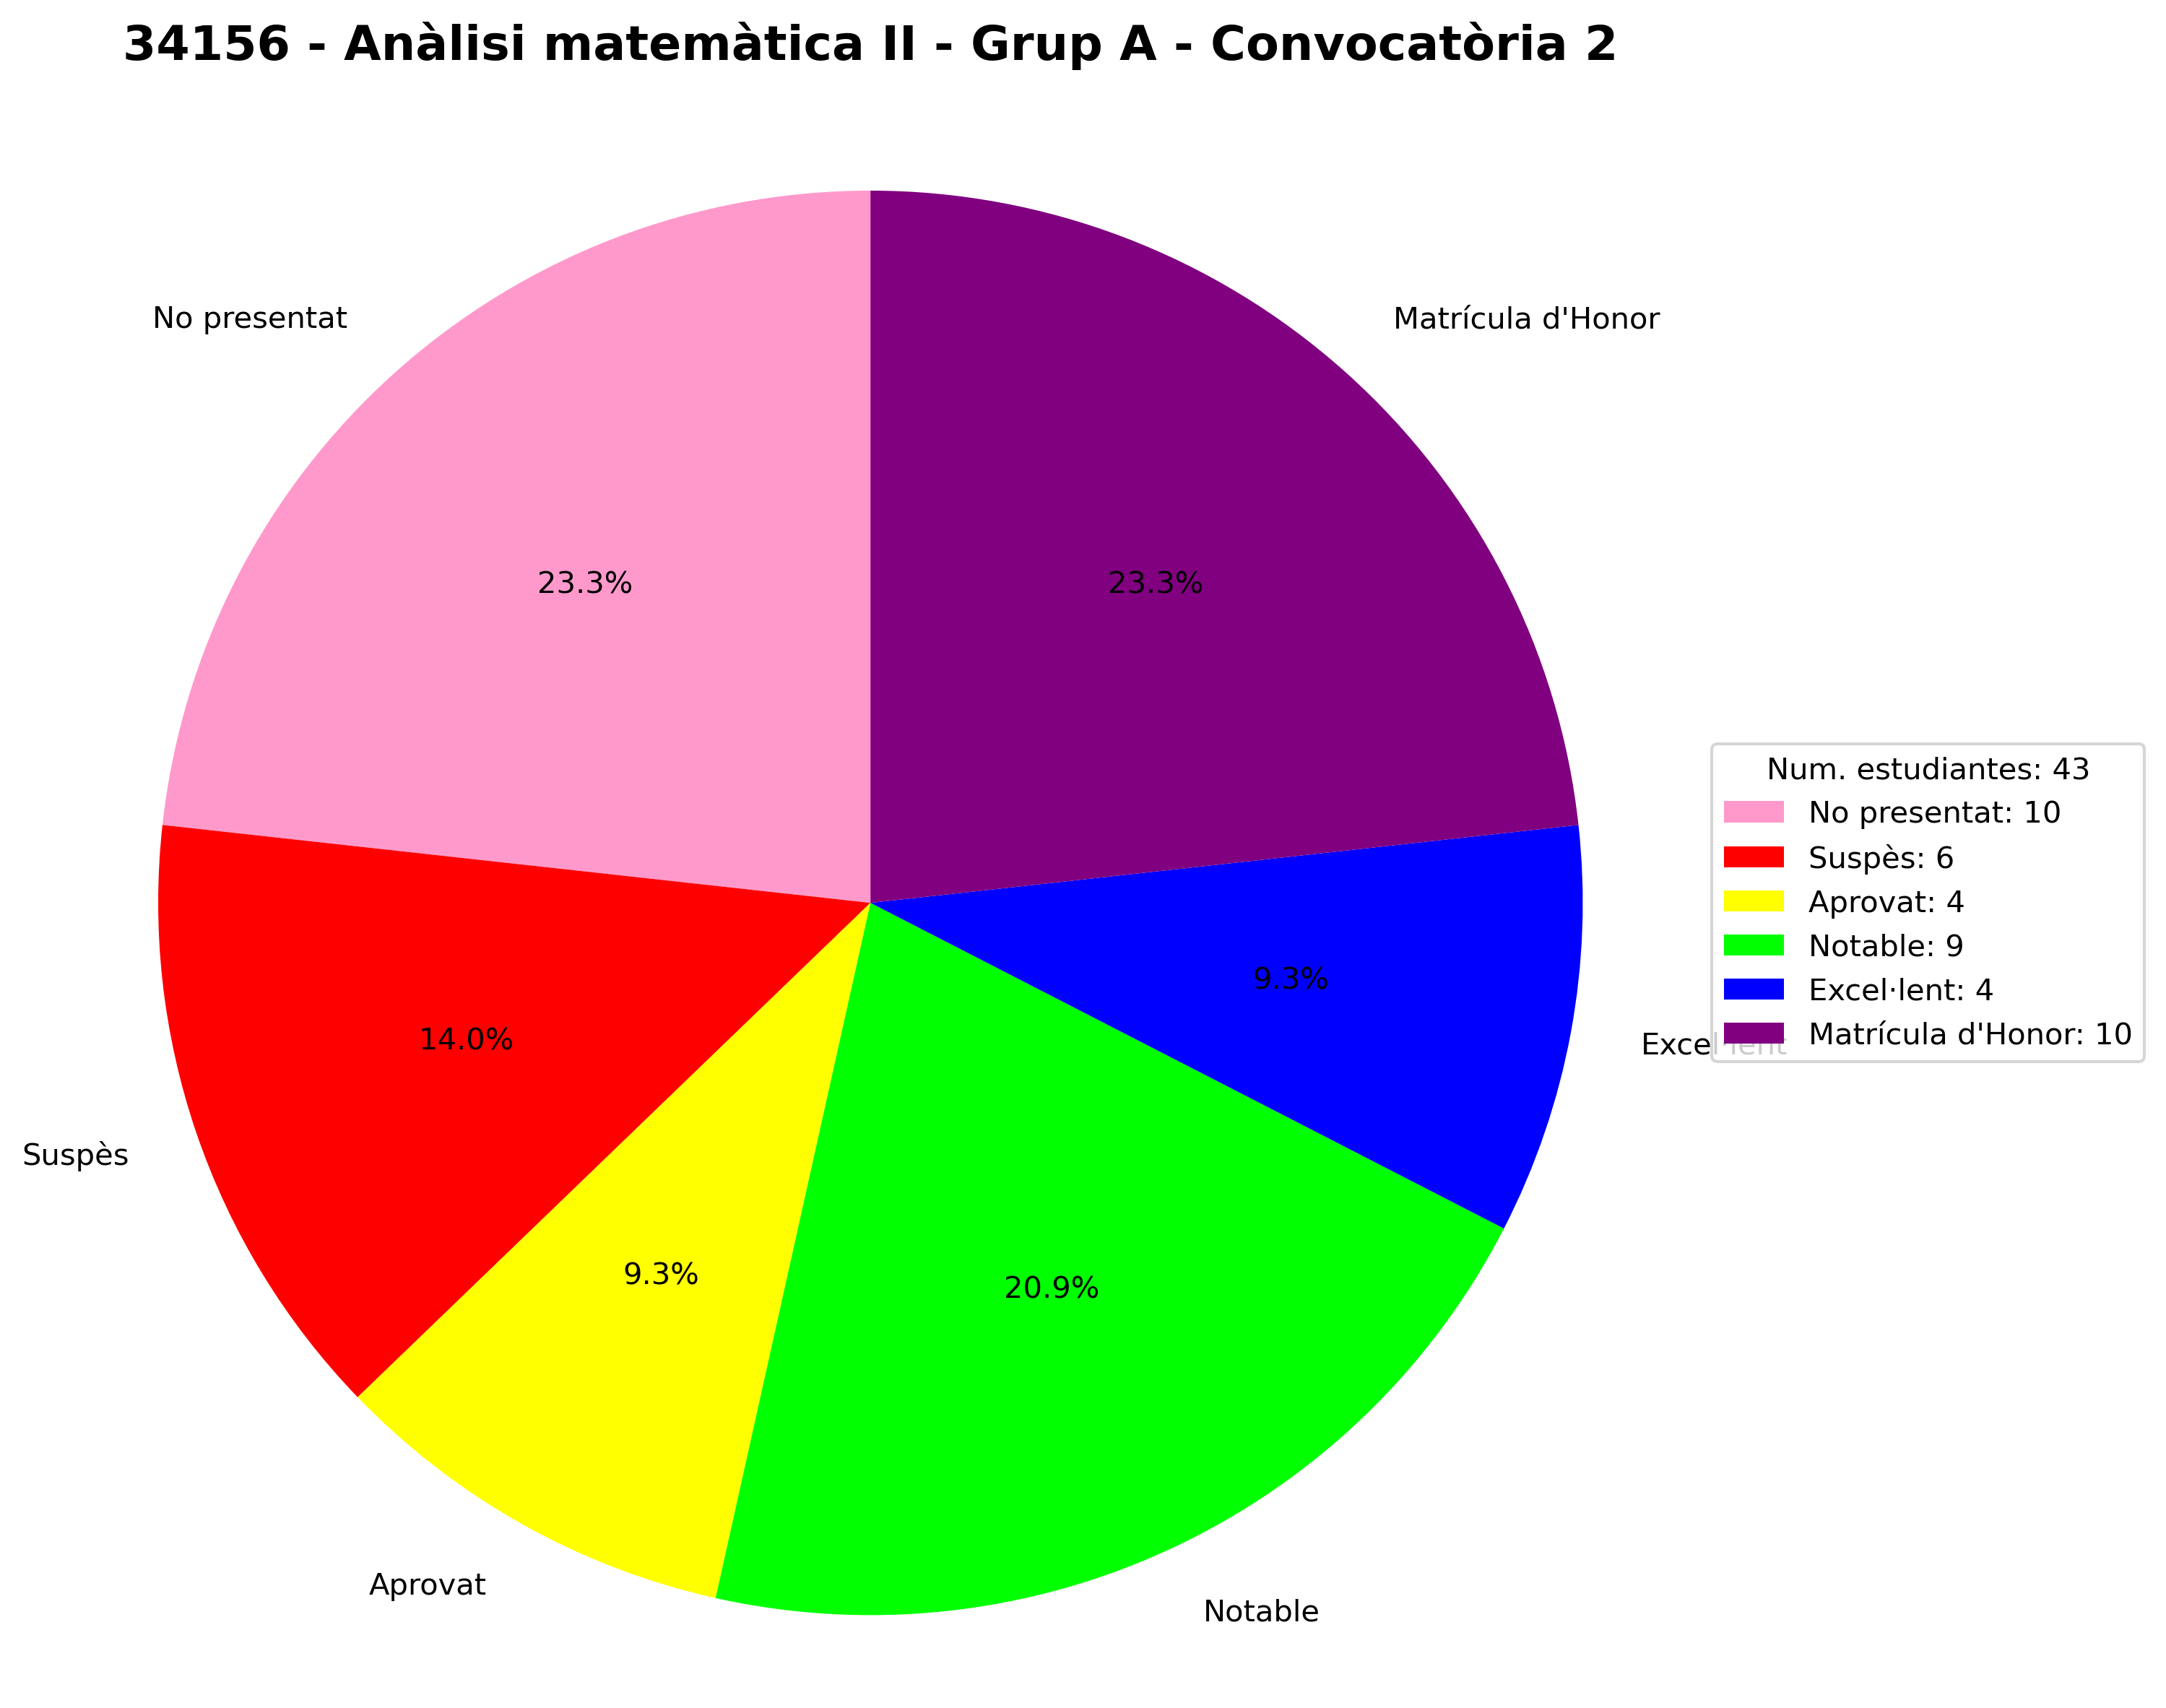
\includegraphics[width=0.8\textwidth]{graficos/34156_A_A2.png}
\caption{34156 - Anàlisi matemàtica II - Grup A - Convocatòria 2}
\end{figure}

\newpage


\end{document}
